\documentclass[border=7pt, convert={density=300,outext=.png}]{standalone}
\usepackage{tikz}

\usepackage[europeanresistors,americaninductors]{circuitikz}

\begin{document}
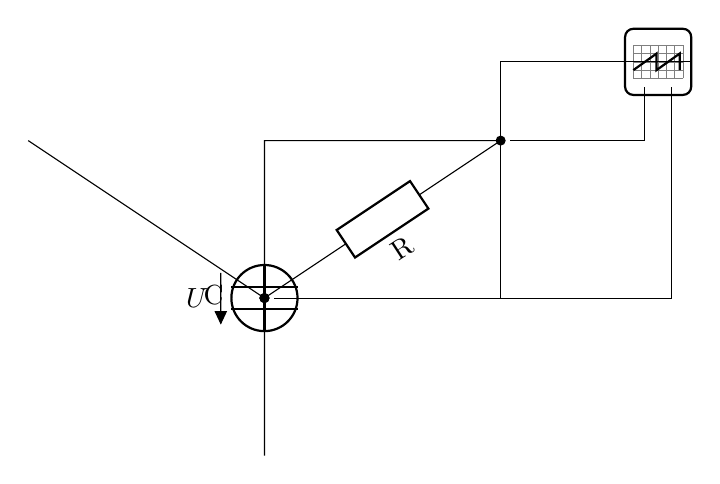
\begin{tikzpicture}

\draw (0,0) to[V,v<=$U$] (0,4) to [short] +(3,0)  node(P_I1){}
    to[R,*-*,l=R] + (0,-2) node(P_I2){} 
    to[C,*-*,l=C] + (0,-2) node(P_I3){} 
    to[short] + (-3,0);

\draw (5,5) node[oscopeshape](O1) {};

\draw (P_I1) -| (O1.in 1);
\draw (P_I2) -| (O1.in 2);
\draw (P_I3) to[short] + (3,0)  |- (O1.east);

\end{tikzpicture}
\end{document}
